\documentclass{ieeeojies}
\usepackage{cite}
\usepackage{amsmath,amssymb,amsfonts}
\usepackage{algorithmic}
\usepackage{graphicx}
\usepackage{textcomp}
\usepackage{array}
\usepackage[table]{xcolor}
\usepackage{multirow}
\usepackage{multicol}
\usepackage{float}
\usepackage[hidelinks]{hyperref}

\def\BibTeX{{\rm B\kern-.05em{\sc i\kern-.025em b}\kern-.08em
    T\kern-.1667em\lower.7ex\hbox{E}\kern-.125emX}}

\begin{document}
\title{FORECASTING STOCK MARKET PRICES USING MACHINE LEARNING AND DEEP LEARNING MODELS}

\author{\uppercase{Ngo van manh}\authorrefmark{1},
\uppercase{Nguyen ngoc thanh\authorrefmark{2}, and Tran Quoc khang}\authorrefmark{3}}

\address[1]{Faculty of Information Systems, University of Information Technology, (e-mail: 21522328@gm.uit.edu.vn)}
\address[2]{Faculty of Information Systems, University of Information Technology, (e-mail: 21522600@gm.uit.edu.vn)}
\address[3]{Faculty of Information Systems, University of Information Technology, (e-mail: 21522200@gm.uit.edu.vn)}

\markboth
{Author \headeretal: Author 1, Author 2, Author 3}
{Author \headeretal: Author 1, Author 2, Author 3}

\begin{abstract}
This paper conducts an analysis and stock price forecasts for VCB, BID, and CTG, the top three banks in Vietnam, crucial entities in the financial sector. These banks play a pivotal role in the country's economic landscape. Leveraging a diverse set of models including Linear Regression, ARIMA, RNN, GRU, LSTM, and N-HITS, we predict both the highest and lowest stock prices of these banks. Furthermore, we employ optimization algorithms such as Nadam and Adadelta to enhance the performance of our Deep learning model and compare when not using optimization models to give insights on efficiency. By scrutinizing stock price fluctuations and employing advanced forecasting methodologies, this study provides valuable insights for investors and stakeholders in the Vietnamese banking industry.
\end{abstract}

\begin{keywords}
Stock price forecasting, Vietnamese banks, VCB, BID, CTG, Linear Regression, ARIMA, RNN, GRU, LSTM, MLP, Nadam, Adadelta.
\end{keywords}

\titlepgskip=-15pt

\maketitle

\section{Introduction}
\label{sec:introduction}
The stock market refers to the collection of markets and ex-change centers where economic activities like buying, selling,and deploying shares of publicly held companies take place.Such financial practices are conducted through institutionalized formal exchanges through over‐the‐counter marketplaces that function under a defined set of regulations. The stock market is a very dynamic and uncertain field, so the stock market prediction naturally becomes a burning topic. Due to the advancement of computational power in recent times, pre-dicting the stock market has been much faster and accurate.Artificial Intelligence and machine learning models play a crucial role in predicting stock prices and, hence, deter-mining an accurate result \cite{b1} \\

This study chooses the Ho Chi Minh Stock Exchange (HOSE) in VietNam, including three different stock market of three VietNamese Banks. There are many algorithms and techniques that help us predict prices. In this paper, we will use Linear Regression, LSTM, RNN, GRU, MLP models to predict the stock prices of VietcomBank, BIDV, VietinBank for the next 30 days \\

\section{Related Works}
This section reviews relevant studies that explore the application of mathematical attributes for stock price prediction. In this study, we will use the following 8 algorithms: Linear regression, ARIMA, RNN, GRU, LSTM, MLP, Nadam, Adadelta to forecast stock prices in Vietnam. In which Nadam \& Adadelta are two optimal algorithms.

\textit{A Multi Parameter Forecasting for Stock Time Series Data Using LSTM and Deep Learning Model}, research by Shahzad Zaheer et al. In this article, they use LTSM, Deep Learning Model to forecast stock prices. But what's special here is that the model takes the original stock data and gives two parameters: closing price and high price for the next day. This proposed method outperforms existing stock price forecasting methods and is considered to be the most accurate and suitable for short-term forecasting. \cite{b2} 

\textit{A Comparative Research of Stock Price Prediction of Selected Stock Indexes and the Stock Market by Using Arima Model}, research by Nayab Minhaj, Roohi Ahmed, Irum Abdul Khalique, Mohammad Imran. This paper explores the use of the ARIMA model for short-term prediction of Johnson \& Johnson (JNJ) stock prices, demonstrating its effectiveness compared to traditional methods. \cite{b3} 

\textit{NHITS: Neural Hierarchical Interpolation for Time Series Forecasting}, research by Cristian Challu et al. In this paper, the author tested large-scale time series datasets for long-term forecasting, demonstrating the advantages of NHITS providing an average accuracy improvement of nearly 20\% compared to the latest Transformer At the same time, it also reduces calculation time. \cite{b4} 

\textit{Nadam: A novel long term solar photovoltaic power forecasting approach using LSTM with Nadam optimizer}, Research by Jatin Sharma et al long-term solar photovoltaic power forecasting using LSTM with Nadam optimizer. The proposed model is compared with two time series models and eight artificial neural network models using LSTM with different optimizers. The obtained results using LSTM with Nadam optimizer present a significant improvement in the forecasting accuracy of 30.56\% over autoregressive integrated moving average, 47.48\% over seasonal autoregressive integrated moving average, and 1.35\%, 1.43\%, 3.51\%, 4.88\%, 11.84\%, 50.69\%, and 58.29\% over models using RMSprop, Adam, Adamax, SGD, Adagrad, Adadelta, and Ftrl optimizer, respectively. \cite{b5} 

\textit{Adelta: ADADELTA: AN ADAPTIVE LEARNING RATE METHOD}, Research by Matthew D. Zeiler. Adadelta is a per-dimension learning rate method for gradient descent, dynamically adjusting rates during training with minimal computation. It eliminates manual tuning and proves robust to noise, different architectures, data types, and hyperparameters. The method shows promising results on MNIST and large-scale voice datasets, effective in both single-machine and distributed settings. \cite{b6} 

\section{Materials and Methodology}
\subsection{Dataset}
The historical stock price of Joint Stock Commercial Bank for Foreign Trade of Vietnam (VCB), Bank for Investment and Development of Vietnam (BIDV) and Military Commercial Joint Stock Bank (CTG) from 01/01/2015 to 27/03/2024 will be applied. The data contains column such as Date, Price, Open, High, Low, Close, Adj Close, Volume. As the goal is to forecast high and low prices, data relating to column “High", "Low" (VND) will be processed.

\subsection{Descriptive Statistics}
\begin{table}[H]
  \centering
  \caption{VCB, BIDV, CTG’s Descriptive Statistics}
    \begin{tabular}{|>{\columncolor{red!20}}c|c|c|c|}
        \hline
         \rowcolor{red!20} 
            High & VCB & BID & CTG \\ \hline
            Count & 2295 & 2301 & 2301 \\ \hline
            Mean & 49,307 & 25,702 & 19,535 \\ \hline
            Std & 22,022 & 10,249 & 6,964 \\ \hline
            Min & 15,779 & 9,172 & 9,707 \\ \hline
            25\% & 25,56 & 15,311 & 13,625 \\ \hline
            50\% & 49,305 & 26,705 & 16,571 \\ \hline
            75\% & 66,293 & 32,385 & 25,819 \\ \hline
            Max & 100,5 & 56,7 & 38,066 \\ \hline
    \end{tabular}
    
    \vspace{10pt}
    
    \begin{tabular}{|>{\columncolor{red!20}}c|c|c|c|}
        \hline
         \rowcolor{red!20} 
            Low & VCB & BID & CTG \\ \hline
            Count & 2295 & 2301 & 2301 \\ \hline
            Mean & 48,157 & 24,956 & 18,997 \\ \hline
            Std & 21,587 & 9,978 & 6,767 \\ \hline
            Min & 15,435 & 9,031 & 9,568 \\ \hline
            25\% & 25,069 & 14,817 & 13,243 \\ \hline
            50\% & 47,778 & 25,753 & 16,051 \\ \hline
            75\% & 64,804 & 31,256 & 25,192 \\ \hline
            Max & 97,3 & 53,5 & 37,303 \\ \hline
    \end{tabular}
\end{table}


\begin{figure}[H]
    \centering
    \begin{minipage}{0.23\textwidth}
    \centering
    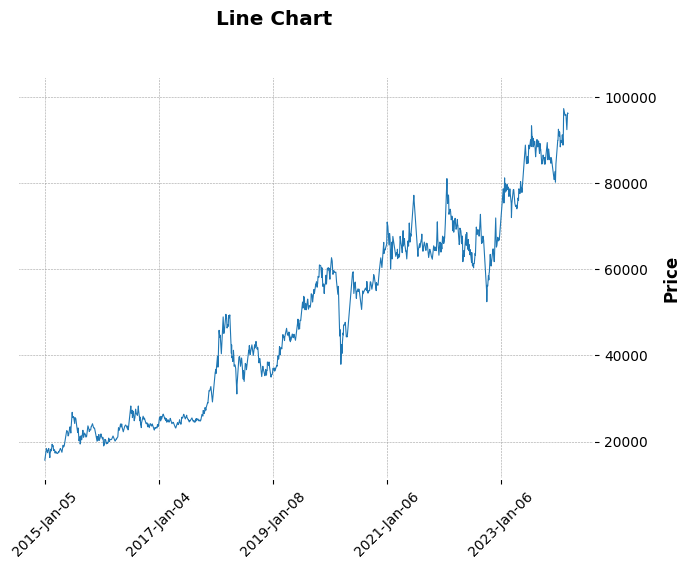
\includegraphics[width=1\textwidth]{bibliography/Figure/vcb_line_chart.png}
    \caption{Vietcombank stock price's line chart}
    \label{fig:1}
    \end{minipage}
\end{figure}

\begin{figure}[H]
    \centering
    \begin{minipage}{0.23\textwidth}
    \centering
    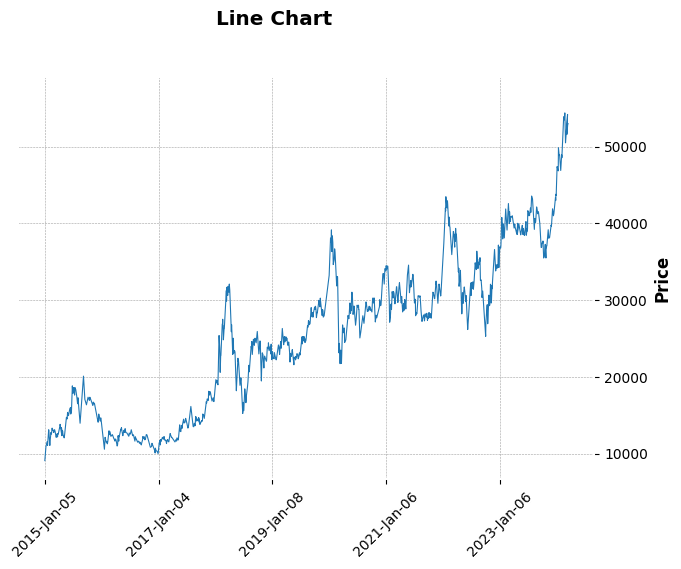
\includegraphics[width=1\textwidth]{bibliography/Figure/bid_line_chart.png}
    \caption{BIDV stock price's line chart}
    \label{fig:1}
    \end{minipage}
    
\end{figure}\begin{figure}[H]
    \centering
    \begin{minipage}{0.23\textwidth}
    \centering
    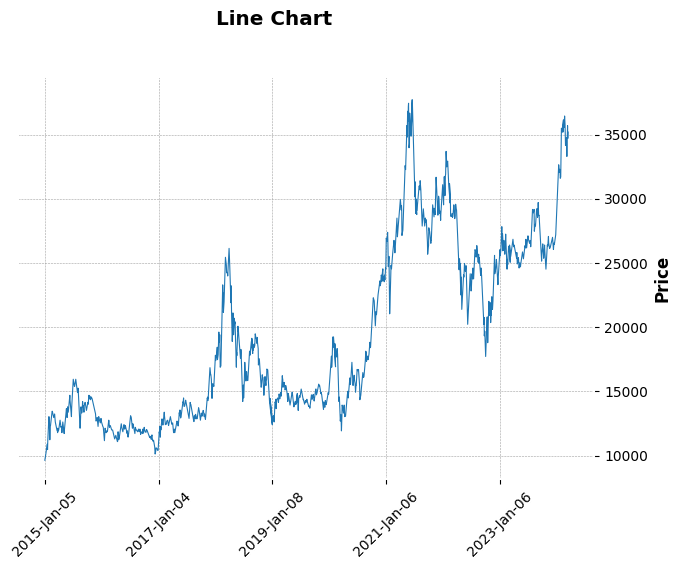
\includegraphics[width=1\textwidth]{bibliography/Figure/ctg_line_chart.png}
    \caption{Vietinbank stock price's line chart}
    \label{fig:1}
    \end{minipage}
\end{figure}
\subsection{Methodology}

\section{Methodology}
\subsection{Linear Regression} 
Regression models are used for describing relationships between variables by fitting a line to the observed data. Regression can estimate how a dependent variable changes as the independent variables change. Multiple linear regression is used for estimating the relationship between two or more independent variables and one dependent variable 
A multiple linear regression model has the form: \cite{b7}
\[Y=\beta_0+\beta_1X_1+\beta_2X_2+\cdots+\beta_kX_k+\varepsilon\]
Where:\\
	\indent\textbullet\ Y is the dependent variable (Target Variable).\\
	\indent\textbullet\ \(X_1, X_2, \ldots, X_k\) are the independent (explanatory) variables.\\
	\indent\textbullet\ \(\beta_0\) is the intercept term.\\
	\indent\textbullet\ \(\beta_1,..., \beta_k\) are the regression coefficients for the independent variables.\\
	\indent\textbullet\ \(\varepsilon\) is the error term.

 \subsection{ARIMA} 
An autoregressive integrated moving average (ARIMA) model is a statistical tool utilized for analyzing time series data, aimed at gaining deeper insights into the dataset or forecasting forthcoming trends. \cite{b8}
\\
\textit{\textbf{Autoregressive (AR)}}
\\
AR is Auto Regression, and p is the number of autoregressive terms . The equation for AR model is: 
\[Y_t = \varphi_1Y_{t-1} + \varphi_2Y_{t-2} + ... + \varphi_pY_{t-p} + \delta + \varepsilon_t\]
\\
\textit{\textbf{Moving Average (MA)}}
\\
MA is the Moving Average, and q is the number of terms in the moving average. The equation for MA model is:  
\[Y_t = \theta_1\varepsilon_{t-1} + \theta_2\varepsilon_{t-2} + ... + \theta_p\varepsilon_{t-p} + \mu + \varepsilon_t\]
\\
\textit{\textbf{Differencing (I) }}
\\
Last, the I part is Integrated, and d is the number of differences (order) required to make it a stationary sequence. For example:
\[If d=0: \Delta Y_t=Y_t\]
\[If d=1: \Delta Y_t=Y_t - Y_{t-1}\]
\[If d=2: \Delta Y_t=\left(Y_t - Y_{t-1}\right) - \left(Y_{t-1} - Y_{t-2}\right)\]
\\
After combining them, we will have the ARIMA (p, d, q) express as follow:
\begin{multline}
\Delta Y_t = \mu + \varphi_1 Y_{t-1} + \varphi_2 Y_{t-2} + \cdots + \varphi_p Y_{t-p} \\
+ \theta_1 \varepsilon_{t-1} + \theta_2 \varepsilon_{t-2} + \cdots + \theta_p \varepsilon_{t-p} + \varepsilon_t
\end{multline}

\subsection{GRU} 
Gated recurrent units(GRU) are a gating mechanism in recurrent neural networks. The GRU is like a long short-term memory (LSTM) with a gating mechanism to input or forget certain features,but lacks a context vector or output gate, resulting in fewer parameters than LSTM.GRU's performance on certain tasks of polyphonic music modeling, speech signal modeling and natural language processing was found to be similar to that of LSTM.
\begin{figure}[H]
    \centering
    \begin{minipage}{0.45\textwidth}
    \centering
    \includegraphics[width=1\textwidth]{bibliography/GRU.svg.png}    
    \label{fig:1}
    \end{minipage}
\end{figure}

\subsection{RNN} 
Recurrent Neural Network(RNN) is a type of Neural Network where the output from the previous step is fed as input to the current step. In traditional neural networks, all the inputs and outputs are independent of each other. Still, in cases when it is required to predict the next word of a sentence, the previous words are required and hence there is a need to remember the previous words. Thus RNN came into existence, which solved this issue with the help of a Hidden Layer.
\begin{figure}[H]
    \centering
    \begin{minipage}{0.45\textwidth}
    \centering
    \includegraphics[width=1\textwidth]{bibliography/RNN.png}    
    \label{fig:1}
    \end{minipage}
\end{figure}
\subsection{LSTM} 
Long Short-Term Memory (LSTM) networks are a specialized type of recurrent neural network (RNN) designed to address the issue of learning from long sequences of data. LSTMs achieve this through memory cells and gates, which regulate information flow, allowing the network to selectively retain or discard information from previous time steps. This selective memory enables LSTMs to effectively model long-term dependencies in sequential data, making them valuable for applications like time series forecasting and natural language processing.
\begin{figure}[H]
    \centering
    \begin{minipage}{0.45\textwidth}
    \centering
    \includegraphics[width=1\textwidth]{bibliography/LSTM.png}    
    \label{fig:1}
    \end{minipage}
\end{figure}
\subsection{MLP} 
Multilayer Perceptrons (MLPs) are a type of artificial neural network with multiple layers of interconnected nodes. They learn through a process called backpropagation, where errors are propagated backward to adjust connection weights and improve predictions. MLPs are versatile tools for tasks like classification, regression, and pattern recognition. However, they can be prone to overfitting and may struggle with vanishing gradients in deep architectures. Despite these limitations, MLPs remain a fundamental building block for many modern deep learning models.
\begin{figure}[H]
    \centering
    \begin{minipage}{0.45\textwidth}
    \centering
    \includegraphics[width=1\textwidth]{bibliography/MLP.png}    
    \label{fig:1}
    \end{minipage}
\end{figure}

\subsection{NADAM} 
Nadam is an optimization algorithm that combines Nesterov momentum and adaptive learning rates. It accelerates gradient descent by looking ahead to where the parameters are likely to be updated. Additionally, it adjusts the learning rate for each parameter based on past gradients. This combination often leads to faster and more stable convergence in neural network training, making it a popular choice for various deep learning tasks.
\subsection{ADADELTA} 
Adadelta optimization is a stochastic gradient descent method that is based on adaptive learning rate per dimension to address two drawbacks:\\
\indent\textbullet\ The continual decay of learning rates throughout training.
\indent\textbullet\ The need for a manually selected global learning rate.

Adadelta is a more robust extension of Adagrad that adapts learning rates based on a moving window of gradient updates, instead of accumulating all past gradients. This way, Adadelta continues learning even when many updates have been done. Compared to Adagrad, in the original version of Adadelta you don't have to set an initial learning rate. In this version, the initial learning rate can be set, as in most other Keras optimizers.



\section{Result}

\subsection{Evaluation Methods}
\[MAPE=\frac{100\%}{n}  \sum_{i=1}^{n} |y_i-\hat{y_i} |  = 1 \]\\
\textbf{Root Mean Squared Error} (RMSE): is the square root of average value of squared error in a set of predicted values.\\
\[RMSE=\sqrt{\sum_{i=1}^{n} \frac{(\hat{y_i}-y_i )^2}{n} }\]\\
\textbf{Mean Absolute Error} (MSLE):is the relative difference between the log-transformed actual and predicted values.\\
\[MSLE=\frac{1}{n}\sum_{i=1}^{n}(log(1+\hat{y_i})-log(log(1+y_i))^2\]
Where: \\
	\indent\textbullet\ \(n\) is the number of observations in the dataset.\\
	\indent\textbullet\ \(y_i\)  is the true value.\\
	\indent\textbullet\ \(\hat{y_i}\) is the predicted value.
\subsection{VCB Dataset} 
% \begin{table}[H]
%     \centering
%     \begin{tabular}{|c|c|c|c|c|}
%          \hline
%          \multicolumn{5}{|c|}{\textbf{VCB Dataset's Evaluation}}\\
%          \hline
%          \centering Model & Training:Testing & RMSE & MAPE (\%) & MSLE\\
%          \hline
%          \multirow{2}{*}{LN} & 7:3 & 10508.77 & 10.71 & 0.015 \\ & 8:2 & 11729.2 & 10.825 & 0.019 \\ & \textbf{9:1} & \textbf{7933.49} & \textbf{7.47} & \textbf{0.007}\\
%          \hline
%          \multirow{2}{*}{SVR} & 7:3&11864.3&7.52&0.021\\ & 8:2&8521.33&5.01&0.009 \\ & \textbf{9:1} & \textbf{7006.54} & \textbf{3.73} & \textbf{0.006}\\
%          \hline
%          \multirow{2}{*}{GRU} & \textbf{7:3}	& \textbf{1545.676} & \textbf{1.262} & \textbf{0.00033} \\ & 8:2 & 1616.817 & 1.267 & 0.00035 \\ & 9:1 & 1699.655  & 1.052 & 0.00032\\
%          \hline
%          \multirow{2}{*}{ARIMA} & 7:3 &  8620.284 &  8.559 & 0.01 \\ & 8:2 &  11729.2 & 10.825 & 0.019 \\ & \textbf{9:1} & \textbf{7644.773}  & \textbf{7.287} & \textbf{0.007}\\
%          \hline
%          \multirow{2}{*}{SARIMA} & \textbf{7:3}	& \textbf{7971.644} & \textbf{7.755} & \textbf{0.009} \\ & 8:2 & 11711.484 & 10.809 & 0.019 \\ & 9:1 & 8629.708 & 8.253 & 0.009\\
%          \hline
%          \multirow{2}{*}{DLM} & 7:3 & 13156.831&13.336 & 0.021 \\ & \textbf{8:2} &	\textbf{7209.84} & \textbf{7.093} & \textbf{0.007} \\ & 9:1 &11945.338	&11.444&0.016\\
%          \hline
%          \multirow{2}{*}{SES} & 7:3 & 10949.0750 & 9.4738 & 0.0169 \\ & 8:2 & 11717.8586 &10.8142 & 0.0189 \\ & \textbf{9:1} &  	\textbf{6000.7953} &	\textbf{5.2412} & 	\textbf{0.004} \\
%          \hline
%          \multirow{2}{*}{BaggingGRU} & 7:3 & 941.7588 &  1.7384 &  0.0005 \\ & 8:2 & 939.7588 &  1.6546 &  0.0005 \\ & \textbf{9:1} & \textbf{936.8374} & \textbf{1.6273} & \textbf{0.0005}\\
%          \hline
%     \end{tabular}
%     \caption{VCB Dataset's Evaluation}
%     \label{vcbresult}
% \end{table}

% Arima model

\begin{figure}[H]
  \centering
  \begin{minipage}{0.8\linewidth}
    \centering
    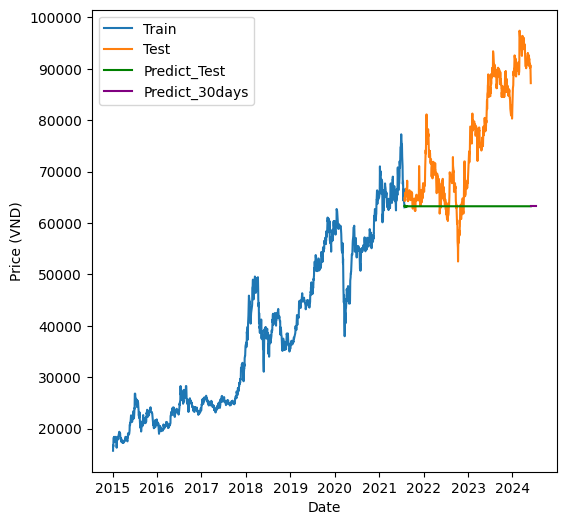
\includegraphics[width=\linewidth]{bibliography/ARIMA/VCB(7-3).png}
    \caption{ARIMA model's result with 7:3 splitting proportion}
    \label{fig8}
  \end{minipage}
\end{figure}

\begin{figure}[H]
  \centering
  \begin{minipage}{0.8\linewidth}
    \centering
    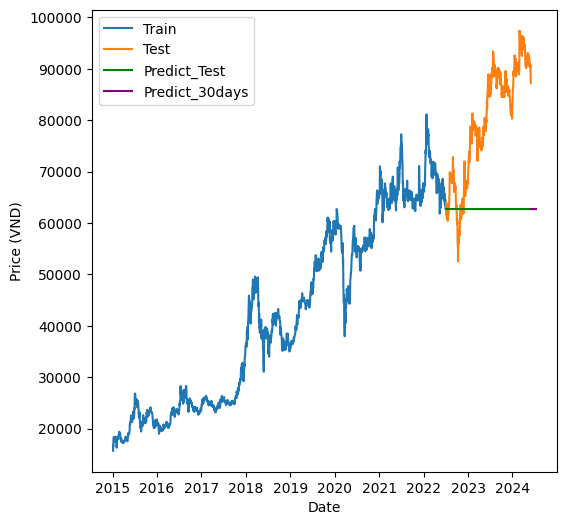
\includegraphics[width=\linewidth]{bibliography/ARIMA/VCB(8-2).png}
    \caption{ARIMA model's result with 8:2 splitting proportion}
    \label{fig8}
  \end{minipage}
\end{figure}

\begin{figure}[H]
  \centering
  \begin{minipage}{0.8\linewidth}
    \centering
    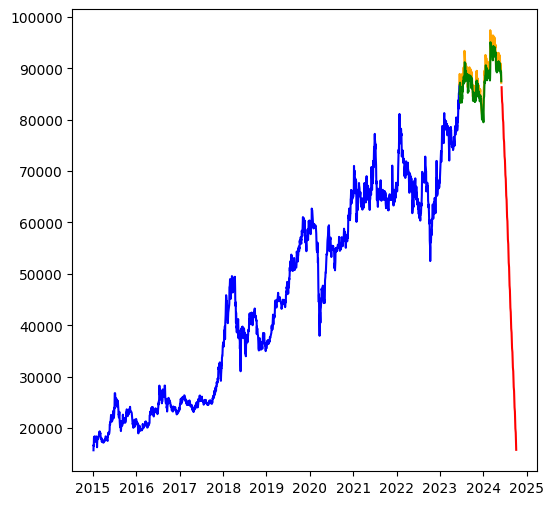
\includegraphics[width=\linewidth]{bibliography/ARIMA/VCB(9-1).png}
    \caption{ARIMA model's result with 9:1 splitting proportion}
    \label{fig8}
  \end{minipage}
\end{figure}

% LSTM

\begin{figure}[H]
  \centering
  \begin{minipage}{0.8\linewidth}
    \centering
    \includegraphics[width=\linewidth]{bibliography/LSTM/VCB 7-3.png}
    \caption{LSTM model's result with 7:3 splitting proportion}
    \label{fig8}
  \end{minipage}
\end{figure}

\begin{figure}[H]
  \centering
  \begin{minipage}{0.8\linewidth}
    \centering
    \includegraphics[width=\linewidth]{bibliography/LSTM/VCB 8-2.png}
    \caption{LSTM model's result with 8:2 splitting proportion}
    \label{fig8}
  \end{minipage}
\end{figure}

\begin{figure}[H]
  \centering
  \begin{minipage}{0.8\linewidth}
    \centering
    \includegraphics[width=\linewidth]{bibliography/LSTM/VCB 9-1.png}
    \caption{LSTM model's result with 9:1 splitting proportion}
    \label{fig8}
  \end{minipage}
\end{figure}

% MLP

\begin{figure}[H]
  \centering
  \begin{minipage}{0.8\linewidth}
    \centering
    \includegraphics[width=\linewidth]{bibliography/MLP/VCB 7-3.png}
    \caption{MLP model's result with 7:3 splitting proportion}
    \label{fig8}
  \end{minipage}
\end{figure}

\begin{figure}[H]
  \centering
  \begin{minipage}{0.8\linewidth}
    \centering
    \includegraphics[width=\linewidth]{bibliography/MLP/VCB 8-2.png}
    \caption{MLP model's result with 8:2 splitting proportion}
    \label{fig8}
  \end{minipage}
\end{figure}

\begin{figure}[H]
  \centering
  \begin{minipage}{0.8\linewidth}
    \centering
    \includegraphics[width=\linewidth]{bibliography/MLP/VCB 9-1.png}
    \caption{MLP model's result with 9:1 splitting proportion}
    \label{fig8}
  \end{minipage}
\end{figure}

% \begin{figure}[H]
%   \centering
%   \begin{minipage}{0.8\linewidth}
%     \centering
%     \includegraphics[width=\linewidth]{bibliography/LSTM/vcb8-2.png}
%     \caption{LSTM model's result with 8:2 splitting proportion}
%     \label{fig8}
%   \end{minipage}
% \end{figure}

% \begin{figure}[H]
%   \centering
%   \begin{minipage}{0.8\linewidth}
%     \centering
%     \includegraphics[width=\linewidth]{bibliography/MLP/MLP_8_2.jpg}
%     \caption{MLP model's result with 8:2 splitting proportion}
%     \label{fig8}
%   \end{minipage}
% \end{figure}

% \begin{figure}[H]
%   \centering
%   \begin{minipage}{0.8\linewidth}
%     \centering
%     \includegraphics[width=\linewidth]{bibliography/LSTM/vcb8-2.png}
%     \caption{LSTM model's result with 8:2 splitting proportion}
%     \label{fig8}
%   \end{minipage}
% \end{figure}
% \begin{figure}[H]
%   \centering
%   \begin{minipage}{0.8\linewidth}
%     \centering
%     \includegraphics[width=\linewidth]{bibliography/SVR_VCB91.png}
%     \caption{SVR model's result with 9:1 splitting proportion}
%     \label{fig9}
%   \end{minipage}
% \end{figure}
% \begin{figure}[H]
%   \centering
%   \begin{minipage}{0.8\linewidth}
%     \centering
%     \includegraphics[width=\linewidth]{bibliography/GRU_VCB73.png}
%     \caption{GRU model's result with 7:3 splitting proportion}
%     \label{fig10}
%   \end{minipage}
% \end{figure}
% \begin{figure}[H]
%   \centering
%   \begin{minipage}{0.8\linewidth}
%     \centering
%     \includegraphics[width=\linewidth]{bibliography/ARIMA_VCB91.png}
%     \caption{ARIMA model's result with 9:1 splitting proportion}
%     \label{fig11}
%   \end{minipage}
% \end{figure}
% \begin{figure}[H]
%   \centering
%   \begin{minipage}{0.8\linewidth}
%     \centering
%     \includegraphics[width=\linewidth]{bibliography/SARIMA_VCB73.png}
%     \caption{SARIMA model's result with 7:3 splitting proportion}
%     \label{fig12}
%   \end{minipage}
% \end{figure}
% \begin{figure}[H]
%   \centering
%   \begin{minipage}{0.8\linewidth}
%     \centering
%     \includegraphics[width=\linewidth]{bibliography/DLM_VCB82.png}
%     \caption{DLM model's result with 8:2 splitting proportion}
%     \label{fig13}
%   \end{minipage}
% \end{figure}
% \begin{figure}[H]
%   \centering
%   \begin{minipage}{0.8\linewidth}
%     \centering
%     \includegraphics[width=\linewidth]{bibliography/ETS_VCB91.png}
%     \caption{SES model's result with 9:1 splitting proportion}
%     \label{fig14}
%   \end{minipage}
% \end{figure}
% \begin{figure}[H]
%   \centering
%   \begin{minipage}{0.8\linewidth}
%     \centering
%     \includegraphics[width=\linewidth]{bibliography/baggingGRU_vcb.png}
%     \caption{Bagging-GRU model's result with 8:2 splitting proportion}
%     \label{bagginggru}
%   \end{minipage}
% \end{figure}
\subsection{BID dataset} 

% Arima model

\begin{figure}[H]
  \centering
  \begin{minipage}{0.8\linewidth}
    \centering
    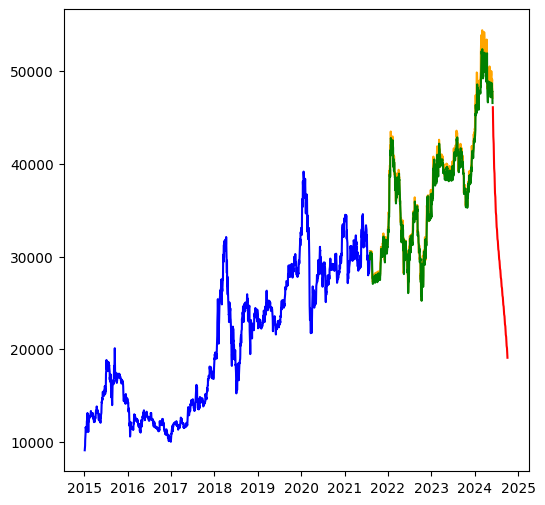
\includegraphics[width=\linewidth]{bibliography/ARIMA/BID(7-3).png}
    \caption{ARIMA model's result with 7:3 splitting proportion}
    \label{fig8}
  \end{minipage}
\end{figure}

\begin{figure}[H]
  \centering
  \begin{minipage}{0.8\linewidth}
    \centering
    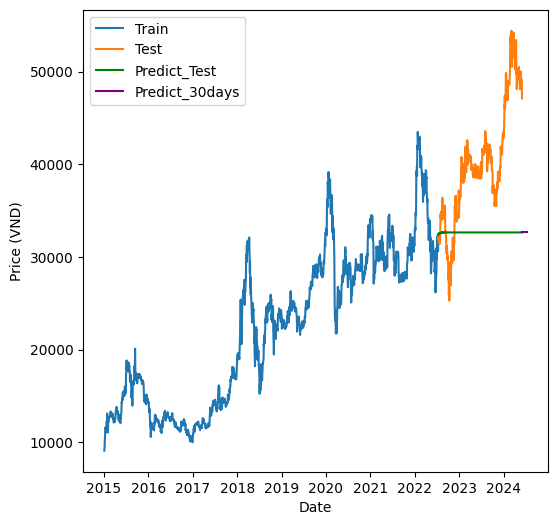
\includegraphics[width=\linewidth]{bibliography/ARIMA/BID(8-2).png}
    \caption{ARIMA model's result with 8:2 splitting proportion}
    \label{fig8}
  \end{minipage}
\end{figure}

\begin{figure}[H]
  \centering
  \begin{minipage}{0.8\linewidth}
    \centering
    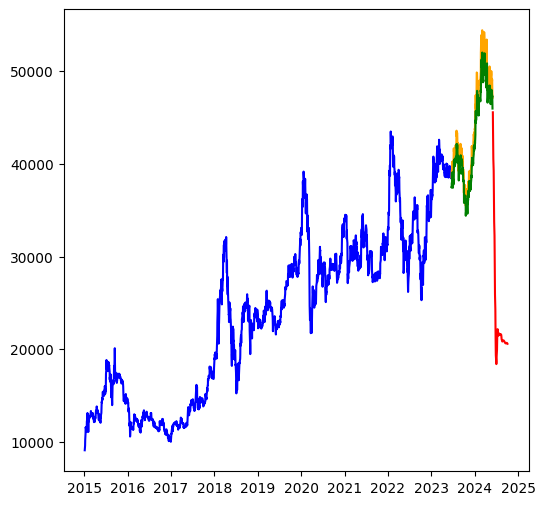
\includegraphics[width=\linewidth]{bibliography/ARIMA/BID(9-1).png}
    \caption{ARIMA model's result with 9:1 splitting proportion}
    \label{fig8}
  \end{minipage}
\end{figure}

% LSTM

\begin{figure}[H]
  \centering
  \begin{minipage}{0.8\linewidth}
    \centering
    \includegraphics[width=\linewidth]{bibliography/LSTM/BID 7-3.png}
    \caption{LSTM model's result with 7:3 splitting proportion}
    \label{fig8}
  \end{minipage}
\end{figure}

\begin{figure}[H]
  \centering
  \begin{minipage}{0.8\linewidth}
    \centering
    \includegraphics[width=\linewidth]{bibliography/LSTM/BID 8-2.png}
    \caption{LSTM model's result with 8:2 splitting proportion}
    \label{fig8}
  \end{minipage}
\end{figure}

\begin{figure}[H]
  \centering
  \begin{minipage}{0.8\linewidth}
    \centering
    \includegraphics[width=\linewidth]{bibliography/LSTM/BID 9-1.png}
    \caption{LSTM model's result with 9:1 splitting proportion}
    \label{fig8}
  \end{minipage}
\end{figure}

% MLP

\begin{figure}[H]
  \centering
  \begin{minipage}{0.8\linewidth}
    \centering
    \includegraphics[width=\linewidth]{bibliography/MLP/BID 7-3.png}
    \caption{MLP model's result with 7:3 splitting proportion}
    \label{fig8}
  \end{minipage}
\end{figure}

\begin{figure}[H]
  \centering
  \begin{minipage}{0.8\linewidth}
    \centering
    \includegraphics[width=\linewidth]{bibliography/MLP/BID 8-2.png}
    \caption{MLP model's result with 8:2 splitting proportion}
    \label{fig8}
  \end{minipage}
\end{figure}

\begin{figure}[H]
  \centering
  \begin{minipage}{0.8\linewidth}
    \centering
    \includegraphics[width=\linewidth]{bibliography/MLP/BID 9-1.png}
    \caption{MLP model's result with 9:1 splitting proportion}
    \label{fig8}
  \end{minipage}
\end{figure}

% \begin{table}[H]
%     \centering
%     \begin{tabular}{|c|c|c|c|c|}
%          \hline
%          \multicolumn{5}{|c|}{\textbf{BID Dataset's Evaluation}}\\
%          \hline
%          \centering Model & Training:Testing & RMSE & MAPE (\%) & MSLE\\
%          \hline
%          \multirow{2}{*}{LN} & \textbf{7:3}&\textbf{4983.47}&\textbf{17.44}&\textbf{0.058} \\ & 8:2 &  5293.6 & 26.28 & 0.063 \\ & 9:1&4894.46&25.85&0.055\\
%          \hline
%          \multirow{2}{*}{SVR} & 7:3&977.55&1.76&0.002 \\ & 8:2&242.75&0.89&0.0002 \\ & \textbf{9:1} & \textbf{162.85} & \textbf{0.75} & \textbf{0.00008}\\
%          \hline
%          \multirow{2}{*}{GRU} & 7:3&454.9923&1.54&0.0005 \\ &  8:2&388.5658&1.406&	0.0005 \\ & \textbf{9:1} & \textbf{373.744} & \textbf{1.36} & \textbf{0.00038}\\
%          \hline
%          \multirow{2}{*}{ARIMA} & 7:3 & 9682.514 & 43.586 & 0.161 \\ & 8:2 & 7136.268 & 36.166 & 0.106 \\ & \textbf{9:1} & \textbf{1139.476} & \textbf{4.57} & \textbf{0.004}\\
%          \hline
%          \multirow{2}{*}{SARIMA} & 7:3 & 9693.439 & 43.648&0.162 \\ &8:2 & 4564.211 & 23.154 & 0.05 \\ &  \textbf{9:1} &  \textbf{1137.416} &  \textbf{4.564} &  \textbf{0.004}\\
%          \hline
%          \multirow{2}{*}{DLM} & 7:3 & 9428.531 & 41.483 & 0.154 \\ & 8:2 & 7054.485 & 34.819 & 0.102\\ & \textbf{9:1} & \textbf{1297.301} & \textbf{5.744} & \textbf{0.005}\\
%          \hline
%          \multirow{2}{*}{SES} & 7:3 &  4988.1456 & 22.7511 & 0.0546 \\ & 8:2 & 4659.5801 & 23.6876 & 0.0516 \\ & \textbf{9:1} &  \textbf{1137.4155} &	\textbf{4.5635} & 	\textbf{0.0036} \\
%          \hline
%          \multirow{2}{*}{BaggingGRU} & 7:3 & 941.7588 &  1.7384 &  0.0005 \\ & 8:2 & 939.7588 &  1.6546 &  0.0005 \\ & \textbf{9:1} & \textbf{936.8374} & \textbf{1.6273} & \textbf{0.0005}\\
%          \hline
%     \end{tabular}
%     \caption{MBB Dataset's Evaluation}
%     \label{mbbresult}
% \end{table}

% \begin{figure}[H]
%   \centering
%   \begin{minipage}{0.8\linewidth}
%     \centering
%     \includegraphics[width=\linewidth]{bibliography/SVR_MBB91.png}
%     \caption{SVR model's result with 9:1 splitting proportion}
%     \label{fig16}
%   \end{minipage}
% \end{figure}
% \begin{figure}[H]
%   \centering
%   \begin{minipage}{0.8\linewidth}
%     \centering
%     \includegraphics[width=\linewidth]{bibliography/GRU_MBB91.png}
%     \caption{GRU model's result with 9:1 splitting proportion}
%     \label{fig17}
%   \end{minipage}
% \end{figure}
% \begin{figure}[H]
%   \centering
%   \begin{minipage}{0.8\linewidth}
%     \centering
%     \includegraphics[width=\linewidth]{bibliography/ARIMA_MBB91.png}
%     \caption{ARIMA model's result with 9:1 splitting proportion}
%     \label{fig18}
%   \end{minipage}
% \end{figure}
% \begin{figure}[H]
%   \centering
%   \begin{minipage}{0.8\linewidth}
%     \centering
%     \includegraphics[width=\linewidth]{bibliography/SARIMA_MBB91.png}
%     \caption{SARIMA model's result with 9:1 splitting proportion}
%     \label{fig19}
%   \end{minipage}
% \end{figure}
% \begin{figure}[H]
%   \centering
%   \begin{minipage}{0.8\linewidth}
%     \centering
%     \includegraphics[width=\linewidth]{bibliography/MLP/MLP_8_2.jpg}
%     \caption{MLP model's result with 8:2 splitting proportion}
%     \label{fig20}
%   \end{minipage}
% \end{figure}
% \begin{figure}[H]
%   \centering
%   \begin{minipage}{0.8\linewidth}
%     \centering
%     \includegraphics[width=\linewidth]{bibliography/ETS_MBB91.png}
%     \caption{SES model's result with 9:1 splitting proportion}
%     \label{fig21}
%   \end{minipage}
% \end{figure}
% \begin{figure}[H]
%   \centering
%   \begin{minipage}{0.8\linewidth}
%     \centering
%     \includegraphics[width=\linewidth]{bibliography/baggingGRU_MBB.png}
%     \caption{Bagging-GRU model's result with 9:1 splitting proportion}
%     \label{mbbbggg}
%   \end{minipage}
% \end{figure}
\subsection{CTG dataset} 

% Arima model

\begin{figure}[H]
  \centering
  \begin{minipage}{0.8\linewidth}
    \centering
    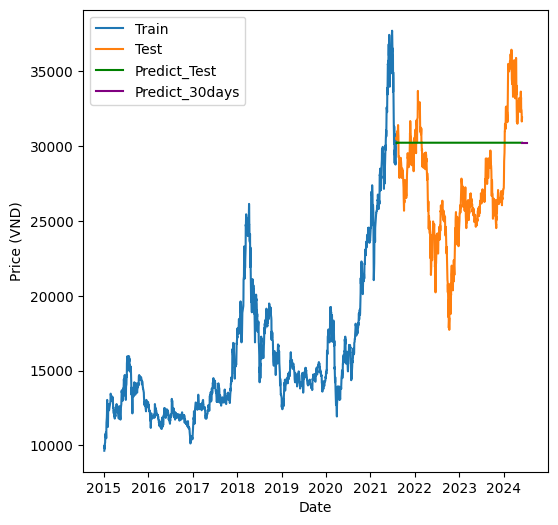
\includegraphics[width=\linewidth]{bibliography/ARIMA/CTG(7-3).png}
    \caption{ARIMA model's result with 7:3 splitting proportion}
    \label{fig8}
  \end{minipage}
\end{figure}

\begin{figure}[H]
  \centering
  \begin{minipage}{0.8\linewidth}
    \centering
    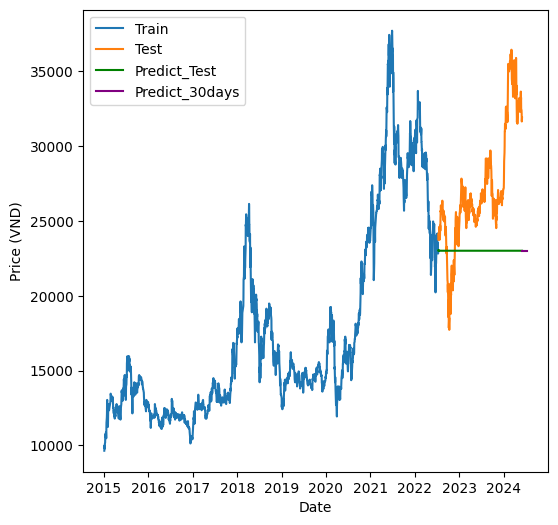
\includegraphics[width=\linewidth]{bibliography/ARIMA/CTG(8-2).png}
    \caption{ARIMA model's result with 8:2 splitting proportion}
    \label{fig8}
  \end{minipage}
\end{figure}

\begin{figure}[H]
  \centering
  \begin{minipage}{0.8\linewidth}
    \centering
    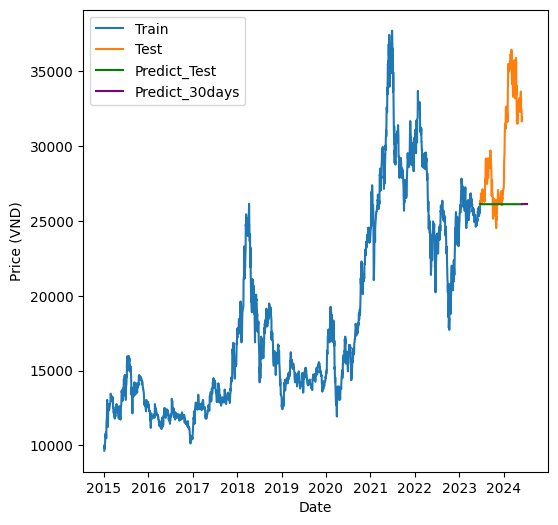
\includegraphics[width=\linewidth]{bibliography/ARIMA/CTG(9-1).png}
    \caption{ARIMA model's result with 9:1 splitting proportion}
    \label{fig8}
  \end{minipage}
\end{figure}

% LSTM

\begin{figure}[H]
  \centering
  \begin{minipage}{0.8\linewidth}
    \centering
    \includegraphics[width=\linewidth]{bibliography/LSTM/CTG 7-3.png}
    \caption{LSTM model's result with 7:3 splitting proportion}
    \label{fig8}
  \end{minipage}
\end{figure}

\begin{figure}[H]
  \centering
  \begin{minipage}{0.8\linewidth}
    \centering
    \includegraphics[width=\linewidth]{bibliography/LSTM/CTG 8-2.png}
    \caption{LSTM model's result with 8:2 splitting proportion}
    \label{fig8}
  \end{minipage}
\end{figure}

\begin{figure}[H]
  \centering
  \begin{minipage}{0.8\linewidth}
    \centering
    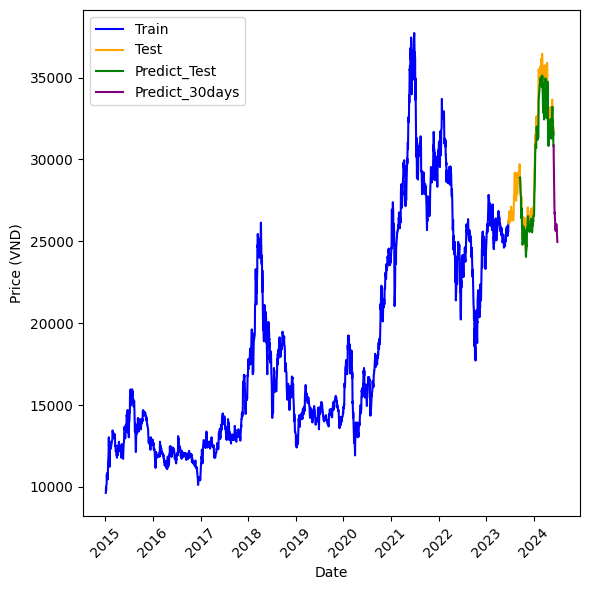
\includegraphics[width=\linewidth]{bibliography/LSTM/CTG 9-1.png}
    \caption{LSTM model's result with 9:1 splitting proportion}
    \label{fig8}
  \end{minipage}
\end{figure}

% MLP

\begin{figure}[H]
  \centering
  \begin{minipage}{0.8\linewidth}
    \centering
    \includegraphics[width=\linewidth]{bibliography/MLP/CTG 7-3.png}
    \caption{MLP model's result with 7:3 splitting proportion}
    \label{fig8}
  \end{minipage}
\end{figure}

\begin{figure}[H]
  \centering
  \begin{minipage}{0.8\linewidth}
    \centering
    \includegraphics[width=\linewidth]{bibliography/MLP/CTG 8-2.png}
    \caption{MLP model's result with 8:2 splitting proportion}
    \label{fig8}
  \end{minipage}
\end{figure}

\begin{figure}[H]
  \centering
  \begin{minipage}{0.8\linewidth}
    \centering
    \includegraphics[width=\linewidth]{bibliography/MLP/CTG 9-1.png}
    \caption{MLP model's result with 9:1 splitting proportion}
    \label{fig8}
  \end{minipage}
\end{figure}


% \begin{table}[H]
%     \centering
%     \begin{tabular}{|c|c|c|c|c|}
%          \hline
%          \multicolumn{5}{|c|}{\textbf{Dataset's Evaluation}}\\
%          \hline
%          \centering Model & Training:Testing & RMSE & MAPE (\%) & MSLE\\
%          \hline
%          \multirow{2}{*}{LN} & 7:3 & 5690.9 & 13.03 & 0.021 \\ & 8:2 & 4904.44 & 10.28 & 0.016 \\ & \textbf{9:1} & \textbf{2859.97} & \textbf{5.49} & \textbf{0.004} \\
%          \hline
%          \multirow{2}{*}{SVR} & 7:3 & 5212.21 & 7.55 & 0.016 \\ & 8:2 & 1014.97 & 1.62 & 0.0005 \\ & \textbf{9:1} & \textbf{822.63} & \textbf{1.26} & \textbf{0.0003}\\
%          \hline
%          \multirow{2}{*}{GRU} & 7:3 & 916.692 & 1.67 & 0.00055 \\ &  8:2 & 948.341 & 1.74 & 0.00057 \\ & \textbf{9:1} &. \textbf{761.754} & \textbf{1.21} & \textbf{0.0003}\\
%          \hline
%          \multirow{2}{*}{ARIMA} & 7:3 & 7847.594 & 15.278 & 0.041 \\ & 8:2 & 7501.223 & 15.14 & 0.036 \\ & \textbf{9:1} & \textbf{3371.058} & \textbf{6.414} & \textbf{0.006}\\
%          \hline
%          \multirow{2}{*}{SARIMA} & 7:3 & 7849.75 & 15.29 & 0.04 \\ &8:2 &7501.73 & 15.15 & 0.04 \\ &  \textbf{9:1} & \textbf{3373.34} & \textbf{6.43} & \textbf{0.006}\\
%          \hline
%          \multirow{2}{*}{DLM} & 7:3 & 4288.68 & 8.641 & 0.012\\ & 8:2 & 3771.703	& 7.756 & 0.009\\ & \textbf{9:1} & \textbf{3617.388} & \textbf{6.446} & \textbf{0.007}\\
%          \hline
%          \multirow{2}{*}{SES} & 7:3 &  7849.6833 & 15.2872 & 0.0407 \\ & 8:2 & 7502.4992 & 15.1483 & 0.0357 \\ & \textbf{9:1} &  \textbf{3342.8102} &	\textbf{6.3561} & 	\textbf{0.0057} \\
%          \hline
%          \multirow{2}{*}{BaggingGRU} & 7:3 & 941.7588 &  1.7384 &  0.0005 \\ & 8:2 & 939.7588 &  1.6546 &  0.0005 \\ & \textbf{9:1} & \textbf{936.8374} & \textbf{1.6273} & \textbf{0.0005}\\
%          \hline
%     \end{tabular}
%     \caption{CTG Dataset's Evaluation}
%     \label{mbbresult}
% \end{table}

% \begin{figure}[H]
%   \centering
%   \begin{minipage}{0.8\linewidth}
%     \centering
%     \includegraphics[width=\linewidth]{bibliography/SVR_BIDV91.png}
%     \caption{SVR model's result with 9:1 splitting proportion}
%     \label{fig23}
%   \end{minipage}
% \end{figure}
% \begin{figure}[H]
%   \centering
%   \begin{minipage}{0.8\linewidth}
%     \centering
%     \includegraphics[width=\linewidth]{bibliography/GRU_BIDV91.png}
%     \caption{GRU model's result with 9:1 splitting proportion}
%     \label{fig24}
%   \end{minipage}
% \end{figure}
% \begin{figure}[H]
%   \centering
%   \begin{minipage}{0.8\linewidth}
%     \centering
%     \includegraphics[width=\linewidth]{bibliography/ARIMA_BIDV91.png}
%     \caption{ARIMA model's result with 9:1 splitting proportion}
%     \label{fig25}
%   \end{minipage}
% \end{figure}
% \begin{figure}[H]
%   \centering
%   \begin{minipage}{0.8\linewidth}
%     \centering
%     \includegraphics[width=\linewidth]{bibliography/SARIMA_BIDV91.png}
%     \caption{SARIMA model's result with 9:1 splitting proportion}
%     \label{fig26}
%   \end{minipage}
% \end{figure}
% \begin{figure}[H]
%   \centering
%   \begin{minipage}{0.8\linewidth}
%     \centering
%         \includegraphics[width=\linewidth]{bibliography/BIDV_DLM91.png}
%     \caption{DLM model's result with 9:1 splitting proportion}
%     \label{fig27}
%   \end{minipage}
% \end{figure}
% \begin{figure}[H]
%   \centering
%   \begin{minipage}{0.8\linewidth}
%     \centering
%         \includegraphics[width=\linewidth]{bibliography/ETS_BIDV91.png}
%     \caption{SES model's result with 9:1 splitting proportion}
%     \label{fig28}
%   \end{minipage}
% \end{figure}
% \begin{figure}[H]
%   \centering
%   \begin{minipage}{0.8\linewidth}
%     \centering
%         \includegraphics[width=\linewidth]{bibliography/baggingGRU_BIDV.png}
%     \caption{Bagging-GRU model's result with 7:3 splitting proportion}
%     \label{fig28}
%   \end{minipage}
% \end{figure}
\section{Conclusion}
After employing six algorithms: ARIMA, Linear Regression,RNN,LSTM, GRU, MLP on three different datasets about stock prices BID, CTG and VCB, we found that the model MLP with Nadam is the best one and gives the best results. superior results based on three measures RMSE, MAPE, MAD on all six algorithms.  
There are also some difficulties such as the training time of 
the model, the number of parameters used, so in the future we 
will improve the model for good and optimal results in terms 
of training time. the number of parameters used,...to 
improved results
\subsection{Summary}
In the achievement of forecasting stock prices, the exploration of diverse methodologies, ranging from traditional statistical models to advanced machine learning algorithms, has been aimed. Among the performed models, Linear Regression (LR), Auto Regressive Integrated Moving Average (ARIMA), Support Vector Regression (SVR), Seasonal Auto Regression Integrated Moving Average (SARIMA), Dynamic Linear Model (DLM), Bagging – GRU, and Simple Exponential Smoothing (SES), it becomes evident that Support Vector Regression (SVR), Gated Recurrent Unit (GRU), and Bagging GRU emerge as the most promising and effective models for predicting stock prices.\\
The intricacies of stock price forecasting, rooted in the complexity and unpredictability of financial markets, demand models that can capture nuanced patterns and relationships within the data. Support Vector Regression (SVR) showcases its efficacy in handling intricate relationships, providing robust predictions. Gated Recurrent Unit (GRU) models, with their ability to capture sequential dependencies, exhibit notable performance in forecasting stock prices. The introduction of ensemble learning through Bagging GRU further refines the predictive capabilities, offering a collective insight that surpasses individual models.\\
As evidenced by the evaluation metrics, including RMSE, MAPE, and MSLE, the SVR, GRU, and Bagging GRU models consistently demonstrate superior performance across various aspects of forecasting accuracy. Their adaptability to handle the inherent uncertainties of stock markets positions them as formidable tools for investors and analysts seeking reliable predictions.
\subsection{Future Considerations}
In our future research, it is crucial to prioritize further optimization of the previously mentioned models. This optimization effort should specifically focus on:\\
\indent\textbullet\ Enhancing the accuracy of the model. While the above algorithms have demonstrated promising results in predicting stock prices, there is a need to further improve the model's accuracy to ensure more precise forecasting outcomes.\\
\indent\textbullet\ Exploring alternative machine learning algorithms or ensemble techniques. Ensemble techniques, such as combining multiple models or using various ensemble learning methods, can also improve the robustness and accuracy of the forecasts.\\
\indent\textbullet\ Researching new forecasting models. The field of forecasting continuously evolves, with new algorithms and models being researched and developed. It is crucial to stay updated with these approaches and explore new forecasting models that offer improved accuracy and performance. \\
By continuously exploring and incorporating new features, data sources, and modeling techniques, we can strive for ongoing optimization of the forecasting models and enhance their ability to predict stock prices with greater precision and reliability.
\section*{Acknowledgment}
\addcontentsline{toc}{section}{Acknowledgment}
First and foremost, we would like to express our sincere gratitude to \textbf{Assoc. Prof. Dr. Nguyen Dinh Thuan} and \textbf{Mr. Nguyen Minh Nhut} for their exceptional guidance, expertise, and invaluable feedback throughout the research process. Their mentorship and unwavering support have been instrumental in shaping the direction and quality of this study. Their profound knowledge, critical insights, and attention to detail have significantly contributed to the success of this research.
\\This research would not have been possible without the support and contributions of our mentors. We would like to extend our heartfelt thanks to everyone involved for their invaluable assistance, encouragement, and belief in our research. Thank you all for your invaluable assistance and encouragement.

%% UNCOMMENT these lines below (and remove the 2 commands above) if you want to embed the bibliografy.
\begin{thebibliography}{00}
\bibitem{b1} 
    Somenath Mukherjee, 
    Bikash Sadhukhan,
    Stock market prediction using deep learning algorithms,
    ResearchGate,   \url{https://www.researchgate.net/publication/354268488_Stock_market_prediction_using_deep_learning_algorithms}
    
\bibitem{b2} 
    Shahzad Zaheer, 
    Nadeem Anjum,
    Saddam Hussain, 
    Abeer D. Algarni, 
    Jawaid Iqbal, 
    Sami Bourouis,
    Syed Sajid Ullah,
    A Multi Parameter Forecasting for Stock Time Series Data Using LSTM and Deep Learning Model,
    \url{https://www.mdpi.com/2227-7390/11/3/590}

\bibitem{b3} 
    Nayab Minhaj, Roohi Ahmed, Irum Abdul Khalique, Mohammad Imran,
    A  Comparative  Research  of  Stock  Price  Prediction  of  Selected  Stock  Indexes and the Stock Market by Using Arima Model, \url{https://ojs.wiserpub.com/index.php/GES/article/view/1426/1046}

\bibitem{b4} 
    Cristian Challu,
    Kin G. Olivares,
    Boris N. Oreshkin,
    Federico Garza Ramirez,
    Max Mergenthaler Canseco,
    Artur Dubrawski,
    NHITS: Neural Hierarchical Interpolation for Time Series Forecasting,
    \url{https://ojs.aaai.org/index.php/AAAI/article/view/25854}

\bibitem{b5} 
    Jatin Sharma1,
    Sameer Soni,
    Priyanka Paliwal,
    Shaik Saboor,
    Prem K. Chaurasiya,
    Mohsen Sharifpur,
    Nima Khalilpoor,
    Asif Afzal,
    A novel long term solar photovoltaic power forecastingapproach using LSTM with Nadam optimizer: A case studyof India,
    \url{https://onlinelibrary.wiley.com/doi/epdf/10.1002/ese3.1178}

\bibitem{b6} 
    Matthew D. Zeiler,
    ADADELTA: AN ADAPTIVE LEARNING RATE METHOD, 
    \url{https://browse.arxiv.org/pdf/1212.5701v1}
    
\bibitem{b7} 
    Rebecca Bevans,
    Multiple Linear Regression, 
    Published on February 20,2020,\url{https://www.scribbr.com/statistics/multiple-linear-regression/}

\bibitem{b8} 
    Duke University,
    ARIMA models for time series forecasting, 
    \url{https://people.duke.edu/~rnau/411arim.htm}

\end{thebibliography}
%%%%%%%%%%%%%%%

\EOD

\end{document}
